\documentclass{scrreprt}

\usepackage{wrapfig}
\usepackage{graphicx}
\usepackage[right=3cm, top=3cm, left=3cm, bottom=3cm]{geometry}
\usepackage[T1]{fontenc}
\usepackage{lmodern}

\begin{document}

\newcommand{\HRule}{\rule{\linewidth}{0.5mm}}
\begin{titlepage}
\begin{center}

% Upper part of the page. The '~' is needed because \\
% only works if a paragraph has started.

\includegraphics[width=0.5\textwidth]{gcu.jpg}~

\includegraphics[width=0.4\textwidth]{lille1.jpg}~\\[3cm]

\LARGE Report
\HRule\\[0.5cm]
% Title
\LARGE 2D Multiplayer Video Game
\HRule\\[1.5cm]

% Author and supervisor
\begin{minipage}{0.4\textwidth}
\begin{flushleft} \large
\emph{Authors:}\\
Carl \textsc{Levasseur},\\
Pierre \textsc{Falez},\\
Benjamin \textsc{Danglot}

\end{flushleft}
\end{minipage}
\begin{minipage}{0.4\textwidth}
\begin{flushright} \large
\emph{Supervisors:} \\
Eddie \textsc{Gray},\\
Mike \textsc{Just},\\
Patrick \textsc{Lebegue}
\end{flushright}
\end{minipage}


\vfill

{\large 2012 - 2013}

\end{center}
\end{titlepage}


\chapter*{Acknowledgments} %TOREWRITE
\addcontentsline{toc}{chapter}{Acknowledgments}
First, we would like to thank Eddie Gray and Mike Just, our supervisors, who have supported us and
gave us lots of advice throughout this project and the Glasgow Caledonian University for
welcoming us and letting us using their comfortable facilities.\\

	  Then, we would also like to thank our French supervisor Patrick Lebegue for supporting us
	  and the University of Lille 1 for giving us the opportunity to carry out our internship in foreign country.\\

	  Finally, we wish to thank all our former professors from the University of Lille 1 who
	  permits us to achieve our graduation in very good conditions.\\

	  \chapter*{Abstract}
	  \addcontentsline{toc}{chapter}{Abstract}
	  During our 3-month-internship at Glasgow Caledonian University, we had to make a video game.
	  In this game, every player have a character, called a hero, which has characteristics, spells, and weapons.\\

	             We made it because it touched to several aspects of computer science such as database, network,
	 	  programming. Moreover, we had to learn a lot of things to get this project done.\\
		  It was also a good opportunity to work in team, and discover what advantages and disadvantages it comes with.
		  We used Git to synchronize our works, and we had a lot of issues about it, but it's part of learning.\\

		  To conclude this abstract we can say that this project was a great experience for many
		  reasons; we had never worked in team before, we learnt to search and develop
		  autonomy. Moreover, as it was an Erasmus placement, we could discover a new country,
		  another language, and last but not least, another culture.

		  \chapter*{Introduction} 
		  \addcontentsline{toc}{chapter}{Introduction}
		  In order to validate our DUT diploma, we choose to carry out our internship in an
		  English speaking country to improve our English language.\\

		  Our supervisor, Eddie Gray, let us choose our project. He gave to us old reports to see what previous students did. He also let us choose technologies to make it.\\

		  We chose to make a 2D Multi-player video game.\\

		  This report consists of four parts. We will first expose the workplace and the project. Then, in a second part, how the application works. Finally, we will describe important technical points.
		  To conclude, we will summarize what this project brought us.\\
	
		  \renewcommand{\contentsname}{Summary}
		  \tableofcontents

		  \part{Project presentation}
		  \chapter{Workplace}
		  \section{Glasgow}%TOREWRITE
		  Glasgow is the largest city in Scotland and third most populous in the United
		  Kingdom. The city is situated on the River Clyde in the country's West Central Lowlands.\\

		 The Industrial Revolution has enabled the 
	   	 region to evolve and Glasgow has become one of the world's pre-eminent center of 
		 engineering and shipbuilding. Moreover it's a student and very warm city. There is a 
		 lot of things to do in Glasgow. There are a lot of museums, parks, and monuments to
		 visit.\\

		  The heart of the city is George Square, located in the city centre, site of many of
		  Glasgow's public statues and the elaborate Victorian Glasgow City Chambers, headquarters
		  of Glasgow City Council.\\

		  Three Universities are present in Glasgow: University of Glasgow, University of
		  Strathclyde and Glasgow Caledonian University.\\

		  \section{Glasgow Caledonian University}
		  Glasgow Caledonian University is a public University. The university was constituted
		  on 1 April 1993 as a result of a merger between Glasgow Polytechnic
		  and The Queen's College. It has 18,500 students from over 100 countries, almost 400
		  different courses available, a modern city-centre campus in Glasgow and high-tech facilities,
		  including the award-winning Saltire Centre library.\\
		  \begin{figure}[h]
		  \begin{center}
		  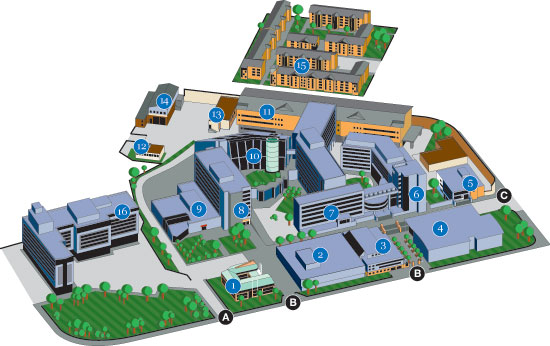
\includegraphics[scale=0.4]{GCU_map.jpg}
		 \caption{GCU map}
		  \end{center}
		  \end{figure}

		  \section{Workspace}
		  The project was mainly realized in our flats because we already had everything we needed there:
		  computers, high-speed Internet connection and softwares. Moreover, we prefered to use our laptops
		  instead of university's computers because our tools were already configured.

		  \chapter{Project definition}
		  The project consists in creating a video game where each player has its own character, also 
		  called a hero. A hero has several characteristics such as speed or strength and can level up by beating his enemies.\\

		  We wanted to do a multi-player video game, on network. Moreover, we want a Role Player Game where the player can truly embodies his character.\\

		  Then, we chose that project because it provides a lot of development opportunities. Unfortunately, we couldn't do everything we wanted to do. Moreover, it was sometimes hard to know what to do in first.\\

		  In fact, at the begin we got lot of ideas:
		  \begin{description}
		  \item[Multi Game Types :]{ First of all, we wanted to implements different game type in order to have a game diversify.}
		  \item[Characters Customizing :] {We also wanted to give the chance to the player to have his own characters, in physical way as well as in skills and spells. Thereby, each character is unique and the player can have a real role-play experience.}
		  \item[Game on network :] {We think online games are better.}
		  \item[Teamwork :] {We wanted to give a real importance to the teamwork. In fact, players have to collaborate with their teammates to win the game.}
		  \end{description}
		  \part{How to play}
		  \chapter{Prerequisite}
		  To be able to launch the application, you must own a MySQL database called '\emph{moba}' with following tables in it:
		  \begin{itemize}
		  \item{account (Account\_ID integer, Account\_Pseudo varchar(32), Account\_Password char(40))}
		  \item{characters (Characters\_ID integer, Characters\_Account integer, Characters\_Name varchar(32) Characters\_Level smallint(6), Characters\_Exp integer)}
		  \item{skill (Skill\_ID integer, Skill\_Characters integer)}
		  \end{itemize}
		
		  You can find this database in the \emph{Database} folder. You just have to import this database in your database management system with few records to get it works.\\

		  To launch the server, you just have to double click on MobaServer.exe, a console should appear showing server's logs.\\
		  It is the same for the client, double click on Moba.exe, but you have to fill \emph{client.conf} with : "server=yourIP". If the server is on the same computer, you don't have to do that.

		  \chapter{Before the game starts}
		  \section{Login screen}
		  \begin{center}
		  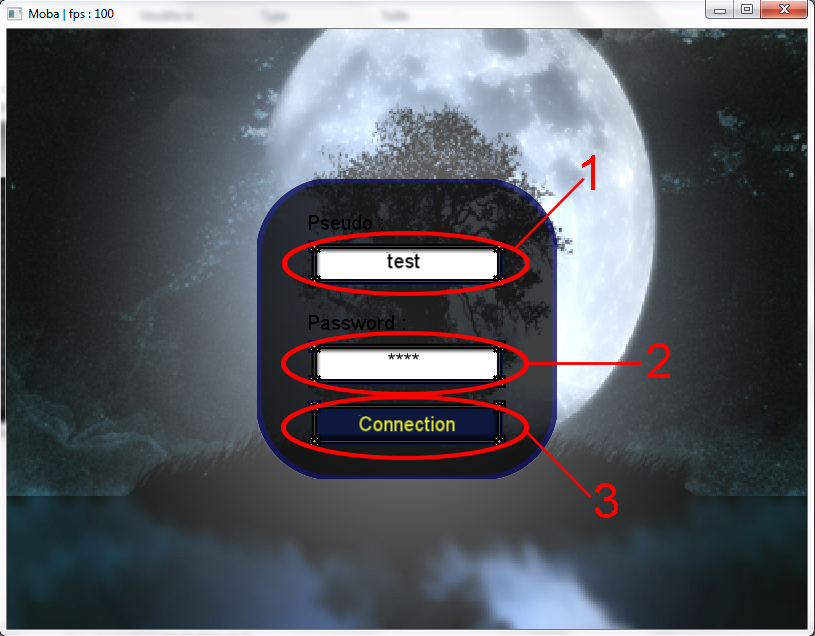
\includegraphics[scale=0.4]{connection_screen.png}
		  \end{center}
		  When you launch the client application, you're invited to connect to the server. To be able to log in, you must have a pseudo and password. Here are few login(1)/password(2) pairs that are already in database:
		  \begin{itemize}
		  \item{test/test}
		  \item{test1/test}
		  \item{test2/test}
		  \end{itemize}

		  Once these fields are filled, click on connection button(3) to connect.
		  
		  \section{Managing your characters}
		  Once you're logged in, you can see the character screen.
		  \begin{center}
		  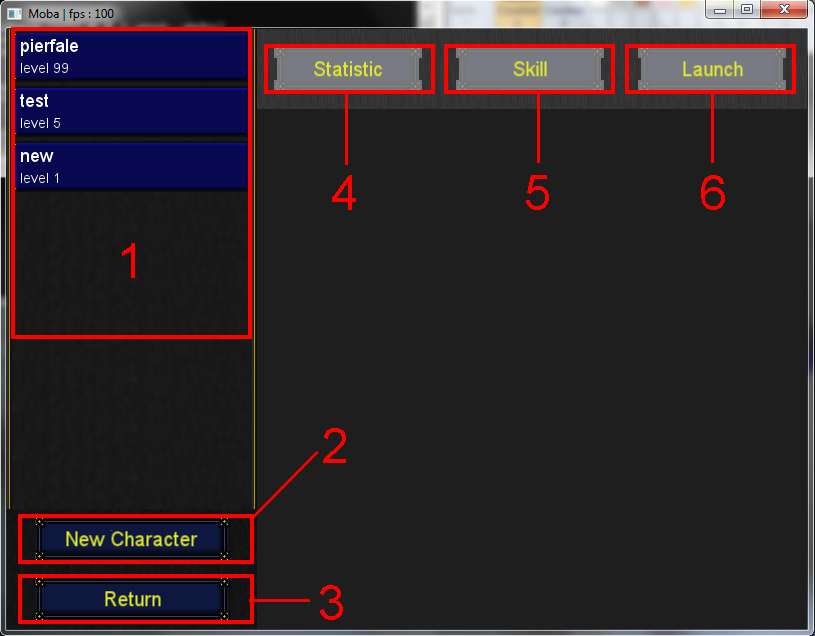
\includegraphics[scale=0.4]{character_screen.png}
		  \end{center}
		  On the left, you have your characters list(1), a 'New character' button to create a new character and 'Return' button(2) to disconnect from server. On the top, you have 3 buttons:
		  \begin{description}
		  \item[Stat(4):]{Display selected character's characteristics}
		  \item[Skill(5):]{Display the skill tree for current character}
		  \item[Launch(6):]{Go to launch screen}
		  \end{description}
		  If you don't have any character yet, you're invited to create a new one.

		  \subsection{Creating a new character}
		  \begin{center}
		  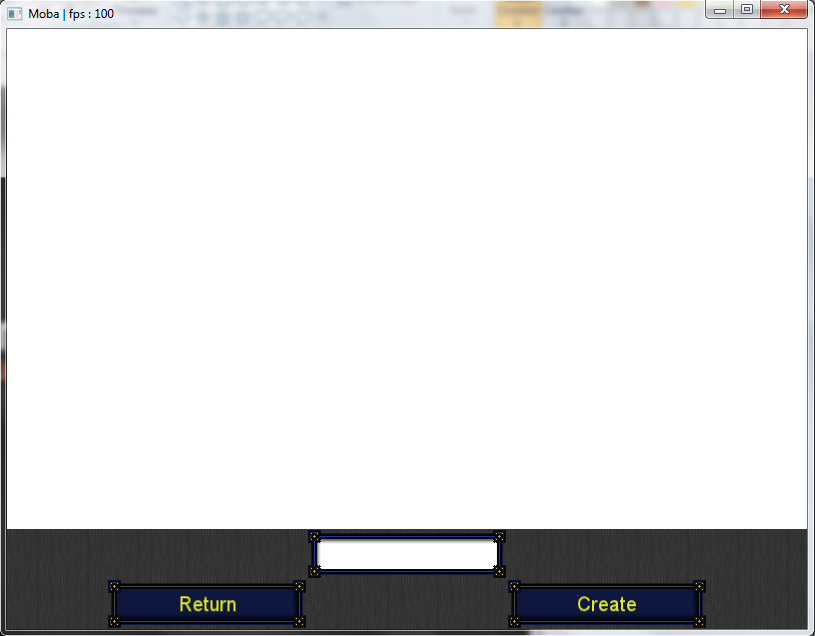
\includegraphics[scale=0.4]{create_character.png}
		  \end{center}
		  We wanted to give the opportunity to customize your character on this screen, but unfortunately, we didn't have enough time and knowledge about graphics, so we only have one skin for all characters. The textfield at bottom of the screen correspond to the name of the character.
		  \subsection{Statistics}
		  \begin{center}
		  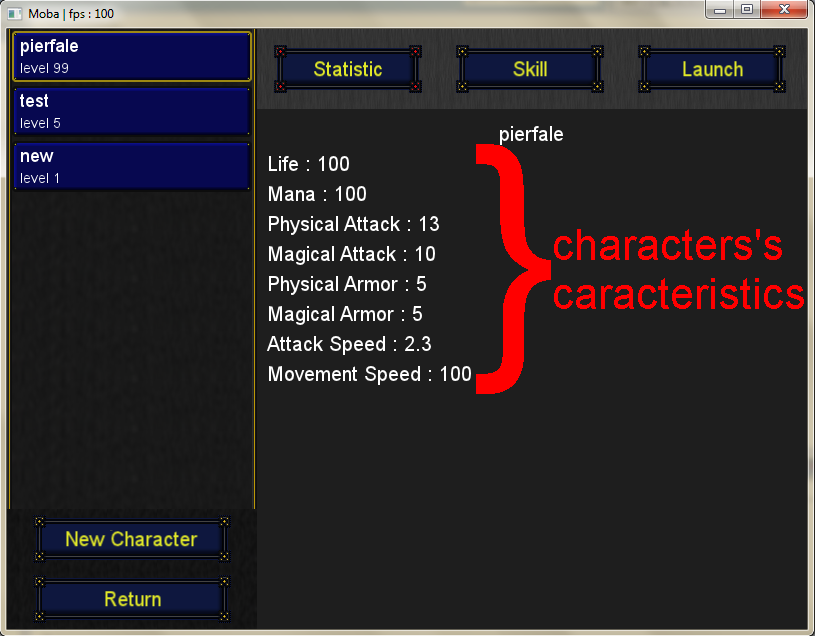
\includegraphics[scale=0.3]{stats_screen.png}
		  \end{center}
		  That screen summarize character characteristics.
		  \subsection{Skill-tree}
		  \begin{center}
		  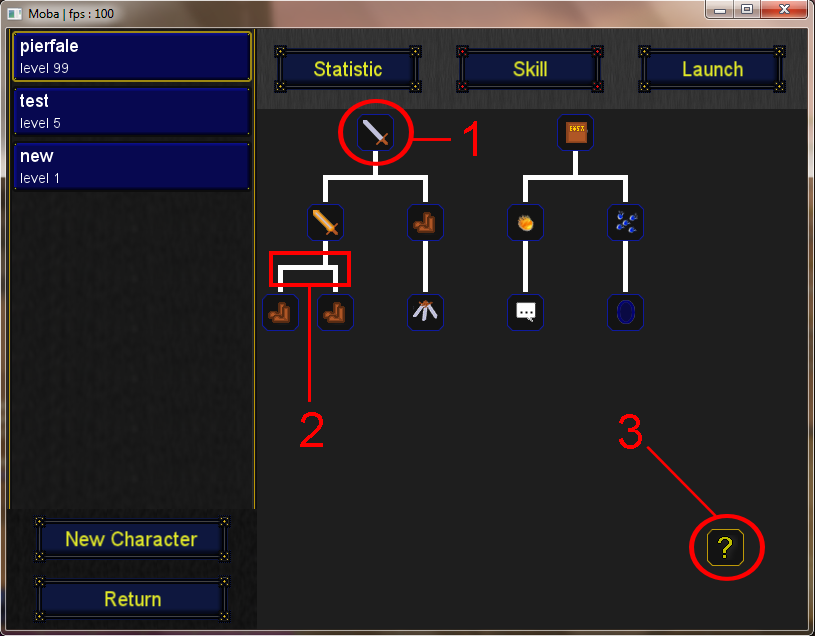
\includegraphics[scale=0.4]{skill_tree_screen.png}
		  \end{center}
		  This is the skill tree screen. Here, you can buy improvements for your character. For each level, you got one point to spend in the tree, but to get a skill, you must get its parent first.
		  \begin{description}
		  \item[Skill(1)]{There is a skill. To buy it, you must have one point and left-click on it. If you can buy it, it appears with yellow borders, if you already bought it, it has blue borders but if you can't buy it, it is dark.}
		  \item[White Lines(2)]{This is the path you must follow. Example : you can not buy \emph{'Powerful Strike'} if you have not buy \emph{'Way of warrior'} first.}
		  \item[Help(3)]{When you put the cursor on it, a tooltip with some help is displayed.}
		  \end{description}
		  \section{Launch a new game}
		  \begin{center}
		  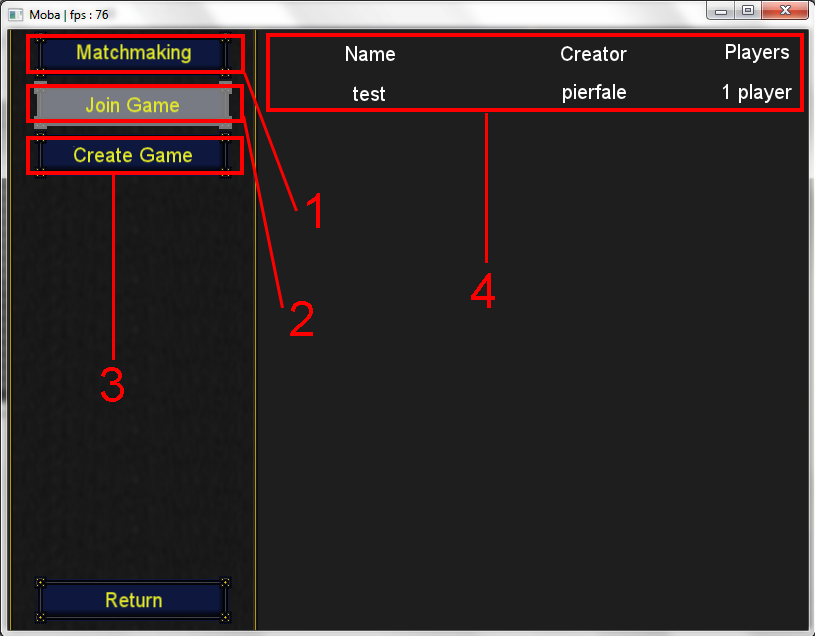
\includegraphics[scale=0.4]{launch_screen.png}
		  \end{center}
		  This screen enables you to create a new game or join an existing one. On the left, there is 3 buttons:
		  \begin{description}
		  \item[MatchMaking(1):]{Search a game where players are at the same level as you, this functionnality isn't implemented}
		  \item[Join Game(2):]{Join a game among those which are available}
		  \item[Create Game(3):]{Create a new game}
		  \end{description}
		  \section{Create a new game}
		  We wanted to give the opportunity to customize your game : game type, time, size of team... But we didn't have enough time to implement it. This screen is similar to the character creation screen. 
		  \section{Join an existing game}
		  \begin{center}
		  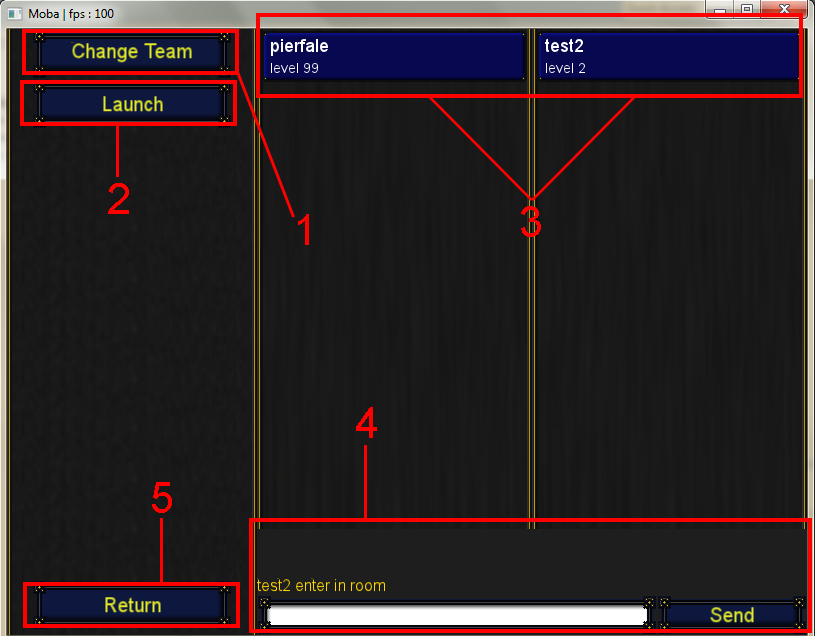
\includegraphics[scale=0.4]{lobby_screen.png}
		  \end{center}
		  This is the screen where teams are created.
		   \begin{description}
		  \item[Change team(1) :]{When you click on this button, your character will change team.}
		  \item[Launch(2) :]{When everyone is ready to launch the game. Only the creator of the game can launch it.}
		  \item[The lobby (3) :]{We can see the two teams, all players and their level.}
		  \item[Chat (4) :]{The chat to speak with other people in this game.}
		  \item[Return (5)] {Go back at the previous screen.}
  		 \end{description}
		  \chapter{In-game}
		  \section{In-game screen}
		  \begin{center}
		  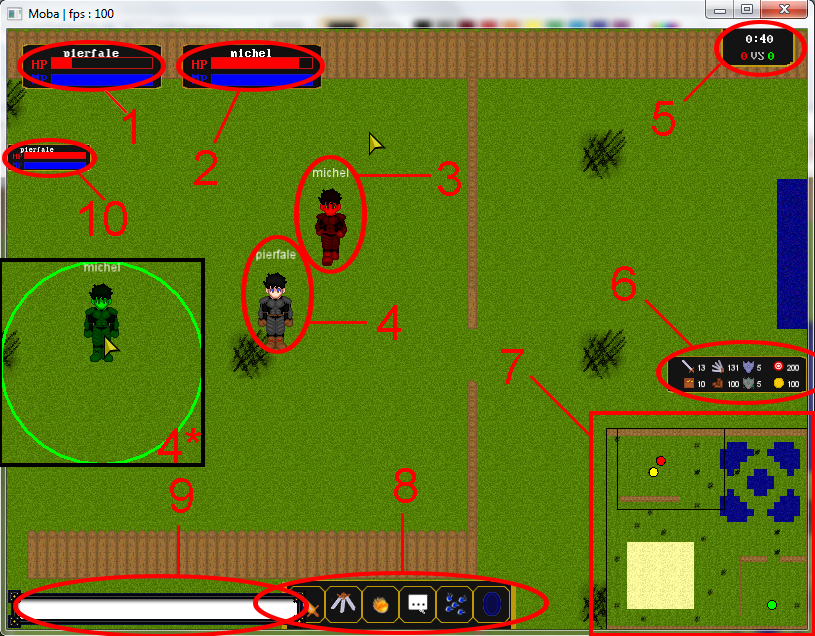
\includegraphics[scale=0.4]{in_game.png}
		  \end{center}
		  The in-game screen is composed of numerous components which display a lot of informations:
		  \begin{description}
		  \item[Character informations(1):]{The HP bar represents character's health (Health points) and the MP bar corresponds to character's mana (Mana points) which are used to cast spells}
		  \item[Target informations(2):]{Same as (1) but corresponds to targeted player's informations}
		  \item[Character (3) and (4):]{When the cursor is on an enemy, he becomes red, if it's a friend, he becomes green}
		  \item[Character's range(4*):]{When your cursor is on your character, a circle representing it's maximal range for attack is drawn around him}
		  \item[Game informations(5):]{Elapsed time and score}
		  \item[Character's characteristics(6):]{Contains all charactestics a player have: physical damages, magical damages, attack speed, movement speed, physical armor, magical armor, range, gold.}
		  \item[Mini map(7):]{Enables to get a global view of the entire map. Your character is represented by the yellow point, friends by green points and enemies by red points}
		  \item[Spell bar(8):]{Allows the player to cast spells, spells which are in this bar depend on your skill tree}
		  \item[Chat(9):]{A chat which permits to speak with other players}
		  \item[Friends informations(10):]{Informations about all your friends in the game}
		  \end{description}

		  \section{Movement}
		To move your character, a simple right-click is required. The character will move to the location where you clicked.
		  \section{Attack}
		  \subsection{Auto-attack}
		To attack enemy with the auto-attack, you have to left-click on him.
		  \subsection{Spells}
		\begin{center}
		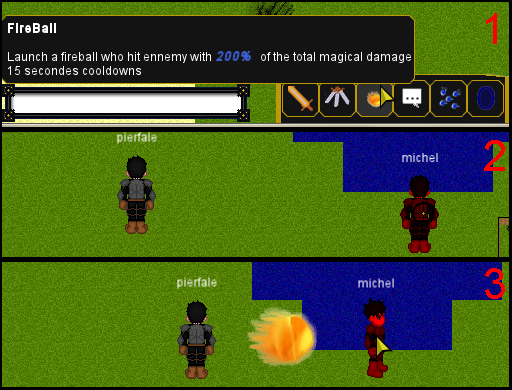
\includegraphics[scale=0.4]{cast_spell.png}
		\end{center}
		To cast a spell, you have to :
 		\begin{description}
  		\item[select a spell(1) :]{click on the spell which you want to launch by a left-click.} 
		\item[target(2) :]{Then the cursor will change and you can target your enemy.}
		\item[fire(3) :]{And with a left-click on the target, the character will cast the spell.}
		 \end{description}
		  \section{Camera}
		To move the camera, you case use arrow keys or put the cursor on the screen's borders.
		  \section{How to win ?}
		There is only one game type available : DeathMatch. Two teams and one goal : have more frags than the other team before the time runs out.
		  \chapter{End-game}
		  \begin{center}
		  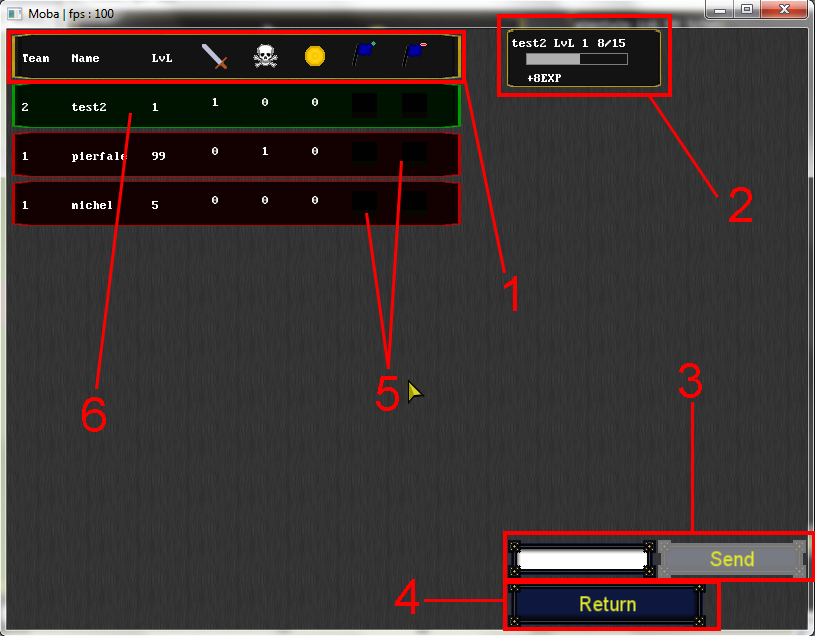
\includegraphics[scale=0.4]{end_screen.png}
		  \end{center}
		  This screen summarizes the game.
		  \begin{description}
		  \item[Header(1):]It is the table's header. There is the team,  characters' names, characters' levels, frags number, deaths number, gold earned, flag captured, flag got back. (gold and flag not implemented yet).
		  \item[Experience(2):]How much experience you earned, and you can see how much experience you still have to earn to level up.
		  \item[Chat(3):] The chat to speak with the other players.
		  \item[Return(4):] to return to the character screen.
		  \item[Enemies' window(5):] In red, we can see informations about our enemis.
		  \item[Allies' window(6):] In green, we can see informations about our allies.
		  \end{description}

		  \part{Technical description}
		  \chapter{Tools}
		  \section{C++}
		  We used C++ all along this project, because it provides interesting libraries for making video games, such as SFML.
		  Moreover, JAVA is the only object-oriented language we studied at the university, so it enabled us to become multi-skilled.
		  Finally, we wanted to try the boost libraries, which allows programmers to make robust C++ programs much more easily, and improve
		  software portability.
		  \section{Eclipse CDT}
		 Eclipse is a multi-language Integrated development environment (IDE) comprising a base workspace and an extensible plug-in system for customizing the environment.\\
		We added the '\emph{CDT}'\footnote{C/C++ Development Toolkit} plugin to code in C++ with Eclipse. We chose Eclipse because we used it before and it provides a very good comfort for coding. But we didn't know that the plug-in didn't work very well and we had some issues with it.
		  \section{Git}
		\begin {center}
		
\includegraphics[scale=0.5]{Git.png}
		\end{center}
		In software development, Git is a distributed version control and source code management (SCM) system with an emphasis on speed.
		We used Git to synchronyze our project faster than with other supports such as USB Key. In fact, we spent a lot of time to merge differents parts of the project at the beginning, but now, we are able to merge a lot of source code in short time.\\
		  \section{External libraries}
		  \subsection{Boost} %TODO
		  \begin{center}
		  
\includegraphics[scale=0.75]{Boost.png}
		  \end{center}
		  Boost is a set of libraries for the C++ programming language that provide support for tasks and structures such as linear algebra, pseudorandom number generation, multithreading, image processing, regular expressions, and unit testing. Release 1.52 contains over eighty individual libraries.\\

		  Most of the Boost libraries are licensed under the Boost Software License, designed to allow Boost to be used with both free and proprietary software projects. Many of Boost's founders are on the C++ standards committee, and several Boost libraries have been accepted for incorporation into both Technical Report 1 and the C++11 standard.

		  \subsection{SFML} %TODO
		  \label{SFML}

		  \begin{center}
		  
\includegraphics[scale=0.75]{SFML2.png}
		  \end{center}

		  SFML (Simple and Fast Multimedia Library) is a portable and easy-to-use API for multimedia programming. It is written in C++ but bindings are available for C, D, Python, Ruby, OCaml, .Net. It is an object oriented alternative for the SDL.\\

		  SFML provides 2D graphics that are hardware accelerated with OpenGL. SFML can also be used for OpenGL windowing. SFML also provides different modules made to ease programming games and multimedia applications. SFML site offers complete SDK bundle in single pack, and tutorials to ease the developers. SFML Source code is provided under the terms of the zlib/png license.

		  \subsection{MySQL}
		  MySQL is the world's most widely used open source relational database management system that runs as a server providing multi-user access to a number of databases. It is also one of the easiest database management system to use, that's why we used it. 
		  \section{Tools we developped} 
		  \subsection{Logs}
		  To make debugging easier, we made a simple log system which redirects the input stream to output stream but also into a file we specified. The class used to do that is called \emph{Logs}. It contains two methods: \emph{out} and \emph{err} which respectively redirect to standard and error streams and the file described by Logs attribute. Also, using a \emph{\#define} macro, we were able to know the file's name and line were Logs methods were called, without having to send it as argument. Thus, we just had to give the message to out or err method.
		  \subsection{Configuration}
		  We also created a basic configuration tool using a parser to extract parameters values from files. Thus, we don't have to compile again each time a parameter is modified. Configuration files must match with the following format:
		  \begin{itemize}
		  \item{Key = value}
		  \item{Key = "value with blanks"}
		  \end{itemize}
		
		  Blanks between \emph{key}, \emph{'='} and \emph{value} are not mandatory
		  It is also possible to put comments into these files by addind a '\emph{\#}' at the beginning of the line. The parser reads each configuration files line by line and stores each key/value pair in a \emph{Map} object. Finally, we developped a class to store default values if none is defined in files, so that we don't have to define a parameter if we want to keep its default value.

		  \subsection{Map editor}
		Maps are handled by a two-dimension-array which contains Case objects. Each Case object contains attributes \emph{x} and \emph{y} to describe its coordinates. Another attribute allow us to know if a character can cross it. Finally, there is an attribute which contains a texture-id so that we know how to paint it. In order to get these maps persistent, we wrote it in binary files. At the beginning, we had to do it manually, but it was tedious to do, so we developped a simple program to make it easier.\\

		Both for performances and ergonomic, we decided to make a map editor, with a texture-palette. Thus, we can create new maps just by using the mouse, with two layers to handle the element overlay, then we can save it and load it into the game. The game display the map by reading its binary file, once it knows the id of each Case, it paints the corresponding texture at Case's coordinates.

		\begin{center}
		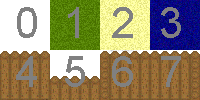
\includegraphics{image1.png}
		\end{center}
		
		\subsection{XML Parser}
		SFML has a class which permits to display text, sf::Text. But the text displayed by this class can only have one style, one color and a one size. In order to solve this problem, we created the \emph{String} class, which inherits from \emph{Component}, and allows us to read XML files. A default style is applied to the text, but we can customize it by adding tags around text portions which we want to put a different style. Here are the tags available:
		\begin{description}
		\item[<b> Text </b>]{Put the text in bold}
		\item[<br/>]{Jump to next line}
		\item[<color=r,g,b> Text </color>]{Change text color}
		\item[<i> Text </i>]{Put the text in italic}
		\item[<size=value>Text</size>]{Change font size}
		\item[<u> Text </u>]{Underline the text}
		\end{description}

		\chapter{Graphics}
		Once we chose to use SFML library (see \ref{SFML}), we had to find an additional library containing components to make user interfaces, because SFML only provides very basic tools, such as drawing rectangles or circles. Many people developped and distributed libraries like this, but most of them are incomplete or contain bugs, that's why we decided to make our own, based on event-driven programming. We also chose to make the graphic part executed by a single thread. We first tried to create thread for each component, but synchronization and concurrent access between them became to hard to manage.

		\section{Overall Functioning} %TODO
		SFML provides a \emph{sf::RenderWindow} object which contains all informations about window and enables us to draw objects which inherit from \emph{sf::Drawable}, or \emph{sf::Vertex} objects, containing vertex from OpenGL library. SFML use an event system to handle any change on the window: mouse movements, clicks, focus and so on.\\

		We created a \emph{graphics::Window} class which wrap sf::RenderWindow. Then we developped an abstract class called \emph{graphics::component} to represent a graphic component. This class contains two methods: \emph{draw} to draw a component, and \emph{event} to deal with events.
		We also created \emph{graphics::Container} class, which can contain several components. It's role is to draw all of its components. graphics::Window object contains a graphics::Container as root component for the component-tree.\\

		While the window isn't closed, the graphics::Window object carries out each of its actions on the same thread. The order used to do these actions is important to make sure that graphic components are working correctly:
		\begin{description}
		\item[Events:]{graphics::Window gets every element which are contained in SMFL events list and check if it is directly concerned by these or not\footnote{whether the window is resized or closed.}}
		\item[Listeners:]{It calls all functions contained in listener-array.}
		\item[Network packets:]{processes packet-list.}
		\item[Check root component:] It checks if temporary root object is different from null. If it is the case, then the old root object is recursively deleted and replaced by the new one. It happens when we want to display another screen.
		\item[Display:]{Calls draw method from the root object.}
		\item[Sleep:]{If there is remaining time before next frame, then the program sleeps during this time.}
		\end{description}

		\begin{center}
		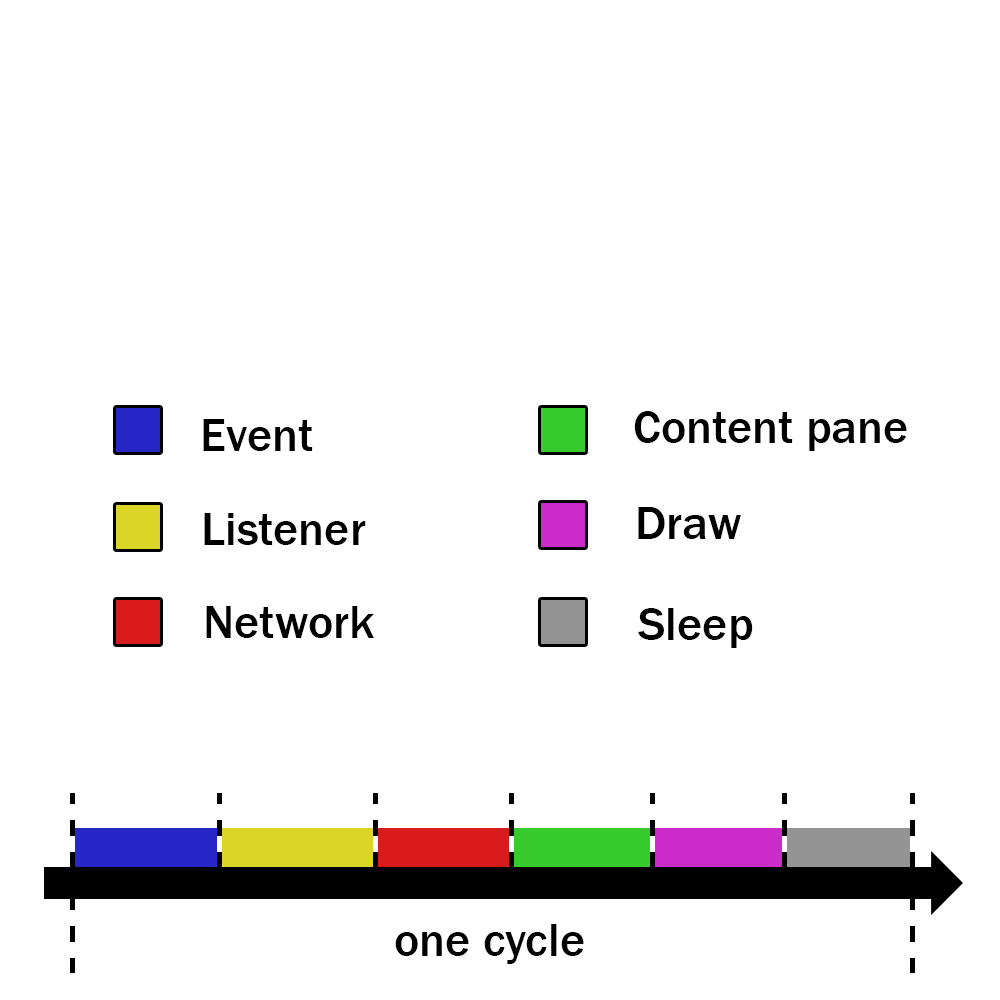
\includegraphics[scale=0.3]{windowCycle.jpg}
		\end{center}

		\section{Components}
		We implemented several essential components to realize this game. They all inherit from \emph{graphics::Component}. This class contains all of their common attributes:
			\begin{itemize}
			\item{Size}
			\item{Position}
			\item{State}
			\end{itemize}

			Their state can be:
			\begin{description}
			\item[normal:]{When the component has no action to do.}
			\item[hidden:]{When the user makes a component hidden, it doesn't respond to events.}
			\item[disabled:]{When the user disables a component, it doesn't respond to events.}
			\item[focused:]{When the user moves his mouse over the component.}
			\item[selected:]{When the user clicks on the component.}
			\end{description}

		  The most important component is \emph{graphics::Container} which inherits from \emph{graphics::Component}. It contains several components and a layout which will situate them whenever the window is resized, or a component is either added, removed or replaced. The graphics::container object spreads a lot of informations to its sons:
		  \begin{itemize}
		  \item{When events are received}
		  \item{How to be displayed}
		  \item{When the graphics::Window is modified}
		  \item{When the component list is modified}
		  \end{itemize}

			Each component must define its own draw and event methods.
			We also have numerous component.

		  \section{Layouts}
		  In order to handle different sizes a window can have, we made several layouts which have to resize and move components following the size of the main window. Each graphics::Container has its own layout instance. The container is expected to destroy the old layout when it is replaced by a new one or when the container itself is destroyed. Every layout inherits from \emph{graphics::Layout} and must define the \emph{validate} method. 
		  The layout knows everything about the container it belongs to, including all of its sons, so it can situate them correctly.
	The default layout included in a container is the VerticalLayout, which aligns all sons vertically and put them at the same size.
We implemented several layouts for all of our needs.

	\section{Events}
	At each frame, the SFML events list is spread as argument to root-container's event method. This method will send these events to all container's sons. It also contains a \emph{used} attribute which allows us to know whether an event has already been transmitted or not so that only one event is triggered when we click on two superimposed components.\\

	Each component handles its events differently, some of them are click-insensitive, others check if the event is sent by keyboard and so on.
	Most components have an \emph{addListener} method which permits to add a new listener. These listeners vary following the component type, a button listener won't be the same as a textfield listener.\\

	When a component wants to call one of its listener's method, it gives the method and listener's reference to the graphics::Window object, which will call them at the right time.

	\subsection{Styles}
	In order to make our components more adaptable, we decided to add classes to change component's style. Each component takes a style object as constructor argument.\\
	The style class changes with the component, for example : Buttons and textfields share the same style: graphics::BasicStyle. This style represents a rectangle : it takes 2 arguments, the path to the border's texture and the path to the center's texture.\\
	We implemented a singleton class to load every style and make easier to put style on component. 
	\section{Modeling characters}
	The characters got three postures : motionless (repeat twice), first step and second step for four directions ( South, East, West, North). We can cut the picture in case : 
	\begin{center}
	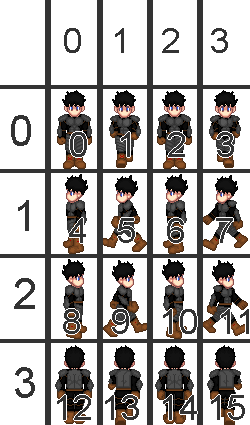
\includegraphics[scale=0.4]{char.png}
	\end{center}
	Each column is a posture, and each row is a direction. With two integers as attributes, we can manage every posture in every direction with a simple addition. For example to have the first step to the north we have :\\
		1 + 3x4 = 13, and the gameboard draw the right "case" of the character's texture.
		\section{Camera}
		The Camera object permits to display a part of map, depending on its position and its range\footnote{the window size}. Thus, the program only draws visible part of the map. We can move the camera either with the directionnal arrows or by moving the mouse on window edges. The movement is done pixel by pixel instead of case by case in order to be more fluid.

		\section{Buffer Y}
		In order to display all components, we use a buffer called \emph{Buffer Y}. At each frame, this buffer is emptied, and is filled with refreshed components (with their new positions, sizes and states). A component must inherit from \emph{graphics::BufferDrawable} to be put in the Buffer Y. This class has two methods:
			\begin{description}
			\item[getvalueY:]{Returns the y-coordinate of the top left where we want to draw the component}
			\item[draw:]{Describes how the component must be drawn}
			\end{description}

			The class which manages the order in which Buffer Y's components should be drawn is \emph{graphics::BufferDraw}. It calls component's draw methods in right order so that we can apply several layers on the window.

			\section{Animations}
			All animations inherit from \emph{graphics::Animation} class which inherits from \emph{graphics::BufferDrawable}. The only attribute an animation owns is '\emph{isDone}', which is true once the animation is finished. To be displayed, an animation object calls \emph{addAnimation} method from the \emph{graphics::GameBoard} class. The gameboard's role is to add all animations which aren't finished, at each frame, to the buffer Y.\\

			Most of animations we implemented are used for spells : the class graphics::SingleTargetSpellAnim, which inherits from Animation, take as argument the caster\footnote{character which cast the spell} and the target of the spell. This class has a static method called \emph{process} which allows to instanciate the right class depending on a spell's id.\\
			Spells' animations are implemented in graphics::SingleTargetSpellImpl. For projectiles, we create graphics::ShotAnim which inherits from graphics::SingleTargetSpellAnim. It is able to determinate the projectile's position with the angle between the caster and the target, and its speed.\\
			There is also LifeLose which displays life points loss.\\
				
				Generally, animations are triggered after a specific packet reception. For example, mono-target spells animations are triggered when a \emph{GAME\_PLAYERLAUNCHSINGLETARGETSPELL} is received, and life loss animation when a \emph{GAME\_DOPHYSICALDAMAGE} has arrived.

				\section{Characters}
				At client side, we splitted the model and view. The model consists of two classes:
				\begin{description}
				\item[game::Character:]{Contains character's id, coordinates, direction and team}
				\item[game::Player:]{Contains character's statistics}
				\end{description}

				On the graphic part, we have:
				\begin{description}
				\item[graphics::Character:]{Inherits from graphics::BufferDrawable}
				\item[graphics::Player:]{Inherits from graphics::Character, which calculates character's position depending on its speed, previous coordinates, direction, and elapsed time since last frame}
				\item[graphics::UserPlayer:]{Inherits from graphics::Player, represents client's character. It handles events in different way and adds some graphic elements. (range in the green circle for example)}
				\end{description}

				About character's movements, we decided to let the client calculates the path to move from its position to the place where the player clicked, to avoid a server overload. However, clients' positions are always checked by the server to make sure they are not cheating. When the client wants to move, it sends GAME\_ASKMOVE) with the number of coordinates and the list of coordinates generated by the pathfinding. Then, for each clients' update, the server calculates the current position and his direction. If client's direction has changed, the server sends to the clients list a packet GAME\_PLAYERMOVE with the client's id, his coordinates and his direction.\\
			The exchange on the network is not instantaneous and different for each client, we had to add an offset on the coordinates calculated by the server in order to make the movement more fluid.\\

			About character's target, the client sends a packet GAME\_ASKTARGET with the target's id, or 0 if it hasn't any target. If the target is okay, the server answer with a packet  GAME\_ANSWERTARGET to confirm.

			\chapter{Network}
			\section{libnetwork}
			Since both the server and the client have network functionnalities in common, instead of writing these function twice, we decided to write a shared library. This library contains the network protocol.\\

				We chose to use TCP as transport protocol because it's more reliable than UDP. Most of datas sent over network needs to be received in the right order by the receiver. To make things easier, most of network functions are executed synchronously, so that we don't have to check all the time if the packet needed to allow the program to continue has arrived or not. Moreover, asynchronous functions use several threads, which increase the program complexity\\

				We defined a basic network protocol to enable clients and server to communicate. Each packet first contains the size of datas that are contained in the packet, on 4 octets, then the packet's type, which is also on 4 octets, and finally all datas. To make packet's type recognition easier, we defined several types in an enumeration: the first eight bits are used to define the packet primary type. Three primary types are available: \emph{Session, Game and Chat}. The three bits remaining are cut in different ways depending on the packet's primary type. This system allows to deal with packets in different classes following the primary type:
				\begin{itemize}
				\item{\emph{SESSION} (0x00 XX XX XX) messages are handled by \emph{Message\_session} class.}
				\item{\emph{GAME} (0x01 XX XX XX) messages are handled by \emph{Message\_game} class.}
				\item{\emph{CHAT} (0x02 XX XX XX) messages are handled by \emph{Message\_chat} class.}
				\end{itemize}

				\section{Server}
				The server is a console application which manages all network packets and helps clients to be synchronized. Its first task during start up is to get its configuration files and parse it. Then, it creates a log file based on its configuration. Once it's done, it loads all informations from the database, such as spells or skills descriptions. Finally, if everything works fine, it binds a socket to the port specified in its configuration and waits for connections.
				\subsection{Access to database}
				To get all necessary datas to make the game work, the server needs an access to a database which contains these informations. That database contains accounts and characters descriptions. We made a \emph{Database} class to execute SQL queries, connect and disconnect from database. If connection to database fails, then the server closes. SQL queries which start with 'SELECT' are handled by a method which return a \emph{ResultQuery} object. This object wrap the MYSQL\_RES structure provided by the MySQL connector and correspond to a row from querie's result. It also contains a \emph{next} method which makes the ResultQuery point to next row and returns true if it exists and false if it doesn't. Finally, it has two \emph{get} methods, the first one takes an integer as argument which corresponds to the column's number, and the second one takes a string as argument which is the name of column we want to get the value.
				\subsection{Connection handling}
				Each client, or connection, is handled in a new thread. Whenever a new connection is opened, a new \emph{Client} object is created on server. This object handles a connection for one client. Then clients and server can communicate.

				\section{How the network protocol is used}
				\subsection{Login}
				Once the thread which handles a connection is created, it waits for a \emph{SESSION\_ASKCONNECTION} packet containing user and SHA1-encrypted password. Then, the server checks if user exists in database and if it's password is the one provided by the client. Following the result of this verification, the server replies with a \emph{SESSION\_ANSWERCONNECTION} packet and one of the following status:
				\begin{itemize}
				\item{NONEXISTENT\_ACCOUNT}
				\item{BAD\_PASSWORD}
				\item{ALREADY\_LOGGED}
				\item{LOGIN\_OK}
				\end{itemize}

				\subsection{Character selection}
				If client is successfuly logged in, it goes to character-selection screen and sends a \emph{SESSION\_ASKCHARACTER} message. Afterwards, the server sends a \emph{SESSION\_ANSWERCHARACTER} for each character the client owns, containing character's id, name, level and experience.\\
					Each Client object contains a \emph{Player} object as attribute. This attribute represents the character chose by client, while the client doesn't select a character, its value is NULL. To update this value, the server must receive a \emph{SESSION\_SELECTCHARACTER} followed by the character id from the client who wants to select a character. The server makes sure that the character exists and is associated to the client before changing the Player attribute's value and load all character's informations from database.

					\subsection{Skills}
					When a client wants to see the tree, it sends a SESSION\_ASKALLSKILLS message. Then, the server replies with a SESSION\_ANSWERALLSKILLS containing the number of skills the client bought and their IDs. The client update its skill-tree afterwards, by circling in blue bought skills, in yellow for those it's allowed to buy, and in grey for those which it can't buy yet.
					When a client wants to buy a new skill, it sends a SESSION\_ASKSKILL packet containing skill ID, if purchase is accepted, the server replies with a SESSION\_ANSWERSKILL, which also contains skill's ID.\\

					For the server, each Player object contains a skill-ID-vector which represents all skills the player owns. To get the informations, the server sends the skill's id. In the SkillImpl class, with the 'process' method, which updates player's statistics and spells. For that, SkillImpl get a map which associates the id to a function containing spell's effects.

					\subsection{Spells}
					Spells are managed in the same way as skills, they are represented by IDs, names, descriptions and icons. During a game launch, the server sends a GAME\_ALLSPELLS packet, containing all spells id and how many they are. Thus, when a client wants to use a spell, he sends a GAME\_ASKLAUNCHSINGLETARGETSPELL, if this spell is mono-target\footnote{A spell which attack only one player}, then the target ID is also included in packet. Then, the server checks several parameters such as target's type, distance between players, and attack/defense bonus applied to each of them, so that it can alter spell's effects correctly. Finally, it sends animation's ID to every player who are in the game.

					\part{Project results}
					\chapter{Encountered difficulties}
					\section{About the project definition}
					We chose a very good project, because it had a lot of things to do in different aspects of computer science. But, with such a project, we got some problems to really define what we wanted to do and with the division of labour.
					\section{About technical aspects}
					We didn't know C++ very well and using git was hard at the beginning. Merging and synchronizing was boring and tedious.
					\chapter{Benefits}
					\section{Programming skills}
					This project enabled us to improve our C++ skills. It gave us a different aspect of object-oriented-language, especially compared to JAVA where most of the work is already done.
					\section{Work in team}
					We learnt to listen to each other, and try to solve our disagreements with compromises in order to satify each teammate. Moreover, we are able to synchronize projects very quickly with Git and now it is very comfortable for us to merge with it.
					\section{English improvement}
					Immersion in Scotland was awesome, and our english skills improved as we wished.
					\section{Autonomy}
					We worked with a great amount of autonomy. The division of labour was the hardest part and even now, each teammate brings something for each project's part.
					\section{Make a report}
					We used \LaTeX  to write this report. It was a great opportunity for us to learn it. \LaTeX is a good tool for writing professional reports.

					\chapter*{Conclusion} %TOREWRITE
					\addcontentsline{toc}{chapter}{Conclusion}
					
					In conclusion, the project is, in our opinion, sucessful. Even if we didn't manage to do everything we wanted, we got a good application.\\
					
					It was a great opportunity for us to make this game, which we may keep improving later. Thus, maybe one day, it will be completed as we expected.\\

					Moreover, we got nice trips, and we could discover Scotland, its people, its landscapes, and its culture.\\
		
					Erasmus is a nice experience for students, we appreciated it. We will advice other students to come to Glasgow.


					\appendix
					\chapter{Components list}
					\addtolength{\oddsidemargin}{-.875in}
					\addtolength{\evensidemargin}{-.875in}
					\small
\begin{center}
\begin{tabular}{|p{2.2cm}|p{4cm}|p{3.5cm}|p{2cm}|p{1.5cm}|p{4cm}|}
\hline
Name & Description & Listener & Style & Selectable & Example \\
\hline
Button & Creates a button, detects clicks and when mouse is mouse is on it & ButtonListener & BasicStyle & true & 
\includegraphics[scale=0.5]{button.png} \\
\hline
ButtonImage & Inherits from Button, allows to put an image on the button & ButtonListener & BasicStyle & true & 
\includegraphics[scale=0.5]{buttonimage.png} \\
\hline
Container & Situates components on window using a layout & None & None & false & 
\includegraphics[scale=0.5]{Container.png} \\
\hline
FocusFrame & Integrated to other components to display a tool tip when the mouse is on it & None & BasicStyle & false & 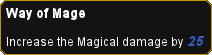
\includegraphics[scale=0.5]{focusframe.png} \\
\hline
InnerWindow & Inherits from Container. Permits to simulate windows inside the main window & InnerWindowListener & WindowStyle & false & 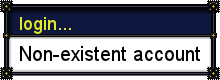
\includegraphics[scale=0.5]{Innerwindow.png} \\
\hline
Label & Used to display text & LabelListener & BasicStyle & false & 
\includegraphics[scale=0.6]{label.png} \\
\hline
Line & Used to display horizontal and vertical lines (for skill tree for example) & None & LineStyle & false & 
\includegraphics[scale=0.5]{Line.png} \\
\hline
ScrollBar & Contains a Container object. If the container is bigger than the scrollBar, then scroll bars are displayed to scroll through the window & None & ScrollBarStyle & false & 
\includegraphics[scale=0.8, angle=90]{ScrollBar.png} \\
\hline
String & Allows to customize texts using XML & None & None & false & 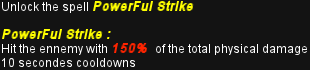
\includegraphics[scale=0.3]{string.png} \\
\hline
Table & Simulates table's behaviour & TableListener & TableStyle & false & 
\includegraphics[scale=0.2]{Table.png} \\
\hline
Textfield & Allows to enter text & TextFieldListener & BasicStyle & false & 
\includegraphics[scale=0.5]{textfield.png} \\
\hline
\end{tabular}
\end{center}
					\chapter{Styles list}
\begin{tabular}{|p{3cm}|p{10cm}|}
\hline
Name & Description \\
\hline
BasicStyle & Takes two images as arguments : The first represents component's borders, the second one represents component's center  \\
\hline
LineStyle & Takes an image as argument to draw the line  \\
\hline
ScrollBarStyle & Takes two images as arguments: the first is the scroll-bar's background, and the second is the bar's image  \\
\hline
StringStyle & Contains all text's personalizations : size, color, italic, underline and bold  \\
\hline
TableStyle & Describes background's color, texts' colors and borders' sizes  \\
\hline
WindowStyle & Similar to BasicStyle but adds an image to represent closing button and parameters to customize window's name  \\
\hline
\end{tabular}

					\chapter{Listeners list}
\begin{tabular}{|p{4cm}|p{10cm}|}
\hline
Name & Methods\\
\hline
ButtonListener & pressed, released, mouseEntered, mouseLeft, selected, unselected, enter \\
\hline
InnerWindowListener & pressed, released, mouseEntered, mouseLeft \\
\hline
LabelListener & mouseEntered, mouseLeft \\
\hline
TableListener & rowSelected \\
\hline
TextFieldListener & textChanged, mouseEntered mouseLeft, selected, unselected, enter \\
\hline
\end{tabular}

\chapter{Database MCD and MLD}
		  \begin{figure}[h]		
		  \begin{center}
		  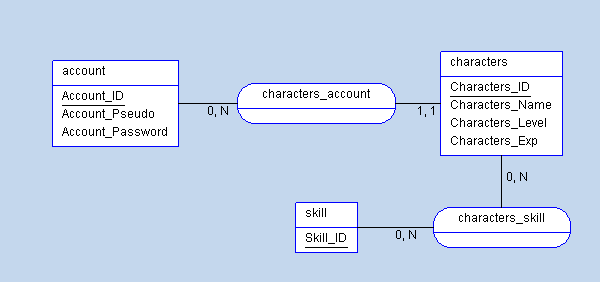
\includegraphics[scale=0.5]{mcd.png}
		  \end{center}
		  \caption{Database MCD}
		  \end{figure}

		  \begin{figure}[h]		
		  \begin{center}
		  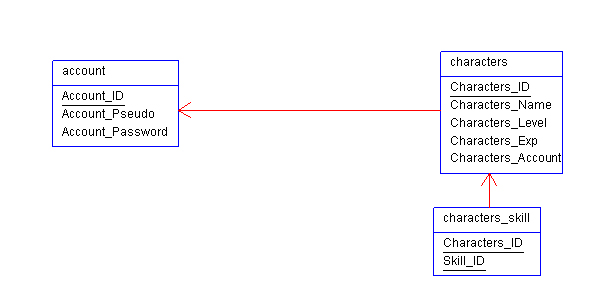
\includegraphics[scale=0.5]{mld.jpg}
		  \end{center}
		  \caption{Database MLD}
		  \end{figure}

\chapter{Links between screens}
		  \begin{figure}[h]		
		  \begin{center}
		  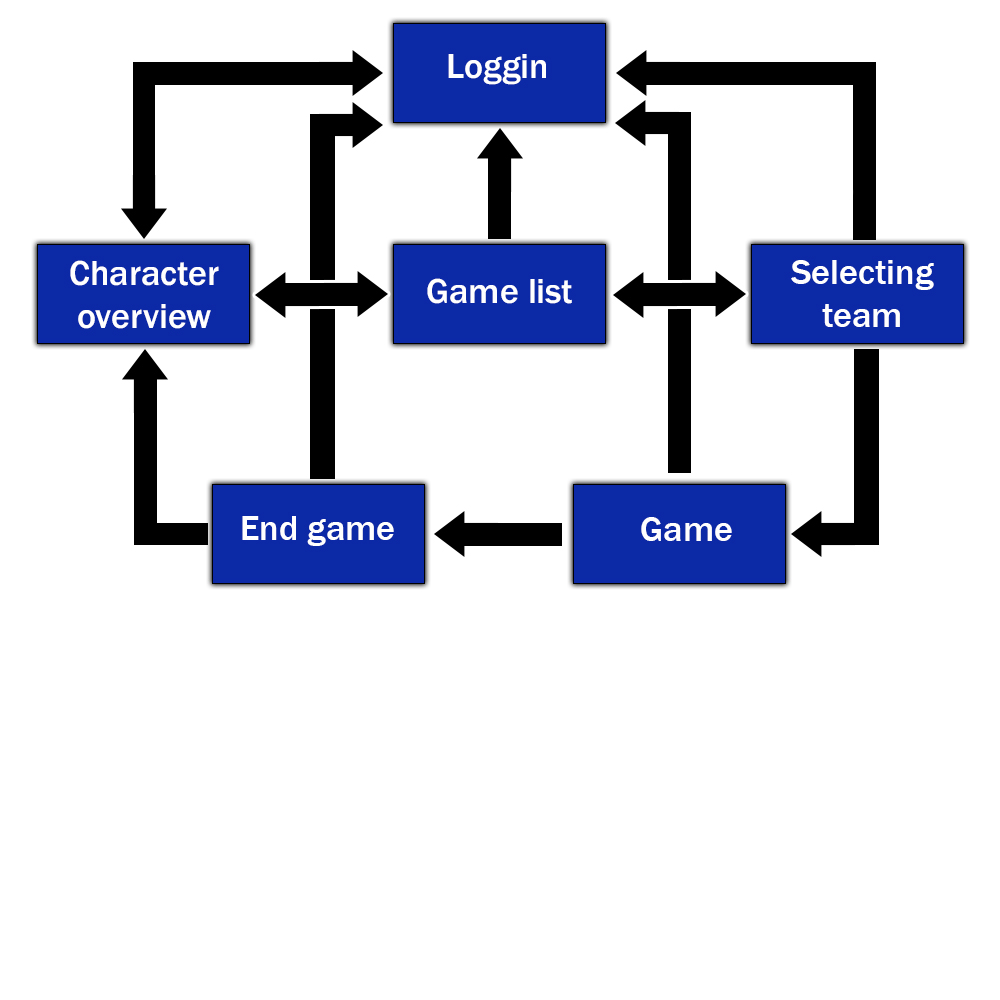
\includegraphics[scale=0.4]{screen.jpg}
		  \end{center}
		  \caption{Screens links}
		  \end{figure}

					\end{document}
